\documentclass[12pt, a4paper]{article}

\usepackage[utf8]{inputenc}
\usepackage[T1]{fontenc}
\usepackage{lmodern}
\usepackage[margin=1.2in]{geometry}
\usepackage{graphicx}
\usepackage{hyperref}
\usepackage{microtype}
\usepackage{setspace}
\usepackage{booktabs}
\usepackage{caption}

\hypersetup{
  colorlinks=true,
  linkcolor=black,
  citecolor=black,
  urlcolor=black
}

\title{A Cognitive Architecture That Produces Teleosemantic Content\\
as Fossilized Wiring Between Independent\\
Perception and Prediction Systems}

\author{Przemys\l{}aw Siemion}
\date{}

\begin{document}

\maketitle

\begin{abstract}
We propose a cognitive architecture in which perception and prediction
are strictly independent systems with no shared vocabulary and no
pre-established correspondence. A matching process, driven by prediction
error, perceptual coverage, and available model capacity, searches for
productive wirings between the two. Successful wirings are retained ---
fossilized --- as the system's ontological commitments. The routing is
the ontology.

This design has consequences: the matching process requires a working
substrate --- a proto-ontology --- without which perception and prediction
cannot be connected. This intermediate structure is not designed into
the system. It is the minimal precondition for the matching problem to
be solvable. The implementation made it necessary before any theoretical
argument.

The architecture re-discovers Millikan's teleosemantics: meaning is
constituted by the consumer's success conditions, and fossilized wiring
is its computational instantiation. Symbol grounding, in this framework,
is not a relation between symbol and world --- grounding comes from
predictive success. The search goes over hypothesis spaces that are
derived, not prescribed.

When the environment changes beyond an incumbent model's capacity, the
architecture supports model succession: competing predictive models,
wired to the same perception stream, provide a basis for ontological
shift as an inspectable architectural event. The system distinguishes
between environments that require extending existing wirings and those
that demand replacing them. What got wired can get re-wired --- from
within.
\end{abstract}

\section{The Problem}

In spite of enormous advances in practical AI applications, a
decades-old problem persists: today's best AI systems, even when
presented with the most compelling evidence, have no mechanism for
revising their ground truths without re-training.

This is not surprising. Ontological shift has been studied at length
and described in depth, but never mechanized. The same unresolved
element has been described by, inter alia, Kuhn in science, Quine in
conceptual schemes, and Piaget in development. Yet no convincing and
realistic mechanism that could realize the ontological shift has been
offered.

The problem cannot be resolved within the framework of Symbolic AI, nor
within end-to-end learning, for seemingly different, but related reasons.
In Symbolic AI, the ontology is given by the designer. In end-to-end
training, ontology is dissolved into weights. Neither of these systems
has the ability to reconfigure itself from the inside.

In this paper we propose a third architecture, in which perception is
separate from predictive machinery. They share neither any a priori
common vocabulary nor any pre-established correspondence. Biologically,
the design principle is to minimize the innate correspondence. The
cognitive effort goes into identifying mappings, or wirings, between
perception and prediction that are successful in giving correct
predictions. Ontological structure emerges as the residue of successful
wiring. Grounding comes from predictive success. Ontological shift may
be interpreted as radical re-wiring. As there is an explicit substrate,
and an explicit process that governs the wiring, everything is
inspectable.

The paper presents the architecture at the computational level in
Marr's sense: some components are conjectured, some have been
implemented and tested, most of them have internal architecture that is
encapsulated and can be explored independently. The architecture is
implementable. A companion paper \cite{companion} demonstrates the architecture at work
in a known minimal-case scenario. We want to stress that many
rectifications of the architecture are coming directly from the
implementation efforts.

\section{The Independence Constraint and the Emergent Ontology}

The first principle of the architecture is that perception and prediction
are two independent systems, and that cognitive processes include, if
not consist of, creating and governing the connections between the two.
Any shared vocabulary, any tight structural coupling, should be avoided
as it violates the principle.

Perception says nothing about what to expect next; prediction has no
sense of ``what'' it predicts. It is the matching process that identifies
the successful mapping between the two, and ``successful'' here has a
very specific meaning: the prediction output, as interpreted by the
wiring, correlates with the successive perception signals.

As perception produces categories in one vocabulary, and prediction
operates in another, the search space is constrained. But the constraint
comes from the vocabulary sizes of the two systems, not from an
externally provided set of hypotheses. This is how the
hypothesis-space problem of Bayesian cognitive science gets resolved by
the architecture: the hypothesis space is effectively the space of
possible wirings.

One consequence of positioning the matching process as the fundamental
actor is that the process needs its working state. This issue became
apparent when working on minimal implementations. The only honest way
to deal with the matching process state is to make it an explicit
component of the architecture. In retrospect we realize it is a catalyst
substrate without which the perception and prediction matching cannot
happen. The initial state of the matching process is assumed to be
blank, but existing. We call it ``proto-ontology.''

The matching process identifies wiring with predictive properties, and
fossilizes this wiring, effectively fusing the emergent ontology onto
its proto-ontology substrate. And as the I/O elements of the prediction
get wired to elements of perception, they, in a sense, assume
\textit{meaning}. But this meaning is emergent, operational, and up
for revisions.

The Independence Constraint is stronger than modularity: modular systems
share interface specifications. Here, no specification exists. The
correspondence is the system's problem to solve.

\section{Architecture}

The architecture is determined by one fundamental idea: interesting
cognitive processes happen \textit{between} perception and the
predictive machinery, and are the only bridge between the two. Defining
minimal meaningful perception and prediction components sets the stage.

\textbf{Perception.} A system that observes a world and produces
discrete perceptual categories. In the simplest version it runs
unsupervised. The architecture does not preclude top-down modulation
from the matching process, but we defer opening this frontier in this
presentation. In effect, the perception system does not need to have
any internal anticipations. Its role is solely to resolve the sensory
inputs onto a vocabulary that is discovered, not specified. It may have
non-trivial internal architecture, but its essential role is to generate
tokens from a slowly-evolving, context-specific vocabulary in response
to external stimuli.

\textbf{Prediction --- a portfolio of predictive models.} Each model is
pre-trained in isolation. Therefore each model is an expert in its
pre-training domain. In this sense, the models do have their internal
ontologies. The crucial point is that the internal ontologies are never
published. There is no labeling that would indicate what the model's
expertise is about. The models' internals remain encapsulated. For this
reason we call them ``boxed models.''

Boxed models expose a homogeneous dictionary, a unified view of their
inputs and outputs. They act as automata driven by signals from the
matcher, and they respond by returning probability distributions over
``next token.''

The distinction between inputs and outputs of a model remains hidden. A
model can have logic based explicitly on some internal semantics --- but
these remain encapsulated and never affect the matcher. This is not just
architectural strictness: being an input or output is a quality
orthogonal to being predictively relevant.

The architecture does not preclude fine-tuning the models once they have
been wired, but, as with the perception modulation, we consider it out
of scope of this paper.

\textbf{The matcher.} The matcher does the cognitive heavy-lifting. It
is the bridge between perception and the predictive models portfolio.

The matcher's task is to establish a productive relationship between
perception and the predictive machinery. It searches the space of
possible wirings between the perception dictionary and the models'
dictionaries. It has an internal measure of predictive error as its
driver. The error function is generic: it simply assesses how probable
the current perception-token is in the latest prediction from the
currently wired model. But because the size and granularity of the
dictionaries is arbitrary, two additional guiding signals are necessary.
One is completeness: are all the world tokens mapped to prediction?
Without this signal the system may have low prediction error because it
quietly ignores some aspects of the perception stream. The other one is
more subtle. It is the model's capacity: it is not necessary that all
the pads of the model are wired. In fact, unwired pads can be considered
a hedge against a changing environment.

The search is oblivious in the sense that the matcher has no other
intrinsic guidelines about which model to wire, and how to map the
dictionaries. The architecture does not constrain the matcher to wire
only one model to the perception.

The quality of a wiring reflects the balance between predictive
accuracy, perceptual coverage, and available capacity. The predictive
error is the main driver, the other two are supportive. What follows is
that, by tuning the relative sensitivities to these signals, the
architecture can approximate different cognitive profiles. For example,
the reactivity to the presence of unwired perception tokens models the
difference between ``dogmatic'' and ``curious.''

The best wiring found is persisted, or ``fossilized,'' because it offers
actual predictive power for the system as a whole. Competing wirings
that perform reasonably may also be retained, as their models' unwired
capacity represents adaptive potential --- a hedge against a changing
environment. The fossilized wirings are all that the system has learned,
and are the only place where any relation between perception and
prediction is retained. A boxed model without wiring is an expert
system. A perception stream without wiring to prediction is just that:
a perception stream. It is our position that profound cognition begins
at the point of connection.

\textbf{Interface principle.} The predictive model never sees raw
perceptual data. It receives signals on its exposed pads from the
matcher, but never knows how its predictions relate to the
\textit{outside}.\footnote{The reader familiar with Stoppard's Dogg's
language will recognize the scenario.}

\section{Grounding as Fossilized Wiring}

Success of the matching process is understood as identifying a wiring
between the vocabulary of perception and vocabularies of one, or more,
predictive models, which results in predictions that are
\textit{useful}. We leave \textit{useful} formally undefined here,
precisely because the concept of usefulness is context-dependent. We
loosely define a \textit{good} wiring as providing a close approximation
of the actual world-token stream.

Once a successful mapping has been established, a wiring exists:
perceptual category X maps to model token Y. ``X is interpreted as Y''
not by representation, not by encoding, but by \textit{routing}. The
routing is the ontology. It has been discovered, it stems from
predictive success, and it is \textit{valuable}. As such, it gets
preserved as a residual trace of a successful matching process.

This way the architecture re-discovers the teleosemantics of Millikan:
meaning is constituted by the success conditions of the consumer, not
by resemblance or stipulation. In Millikan's terms the predictive model
is the consumer, and the wiring's content is whatever has resulted in
the consumer succeeding in predicting the future --- as judged by the
matcher. Fossilized wiring becomes a computational instantiation of the
teleosemantic relation.

This in turn sheds light on the symbol grounding problem, as formulated
by Harnad: how do symbols connect to the \textit{world}? The
architecture walks away from this problem: symbols do not relate
directly to the world. Symbols search for their slots in the predictive
machinery, and their fitness is measured by overall predictive success.
Grounding is contextual, indirect, and it comes from predictive success.

Further: Fodor argues in \textit{Hume Variations} that genuinely new
concepts cannot be acquired --- only triggered from an innate stock. The
architecture half-agrees: predictive models are pre-existing, their
internal vocabulary is not learned from the perception stream. But the
model is not the concept. The concept is a successful application of a
model: good predictive wiring to the world-context. In a departure from
Fodor's ideas, concepts appear to be operational units rather than just
symbols.

There is also a flip side to the operational and emergent nature of
grounding. And this flip side is the architecture's greatest upside:
what got wired, can get re-wired. We tacitly assume such architectures
will adapt. At any point in time the perception stream may change,
partially invalidating the existing predictive power, and triggering a
search for a better, updated matching. A new wiring, to a different
model in the portfolio, may be identified as the new champion and
fossilized. No retraining. No updating of parameters from the outside.
Just changing the routes. From within. Shifting the meanings in an
almost Quinean sense. This is structurally different from Bayesian
belief revision, as it is a change in the interpretation function, not
in the probability distributions.

\section{Model Competition and Succession}

As stated, multiple predictive models can be wired to the same
perception stream simultaneously. The models may be complementary, but
they may also be competitive with one another. The matching process
identifies a winning model, and fossilizes a wiring to it. But the
winner status may be temporary. If the matching process also identifies
one or more other wirings with reasonable predictive performance, they
may be preserved, and their models wired. One reason for keeping these
``contenders'' could be their adaptive potential in the form of their
model's unwired pads.

Let us now describe what we call an ``ontological crisis.'' It is easy
to model a situation in which the external stimuli and the perception
stream change such that the current leading model stops being
satisfactory. It may be that the perception dictionary remains
unchanged, but the current wiring to the current leader's internal
logic does not correlate to perception any longer. It may be that the
dictionary expands, presenting new perception tokens to wire. Or it
could be both.

Heuristically, the third possibility is the most relevant --- the world
rarely changes its internal logic without new factors appearing. It also
offers us the most vivid scenario for model succession.

Assume there is a clear leader in the wiring space --- a wiring that
produces rock-solid predictions. But the wired model is at its capacity,
all its pads have already been tapped. There are also one or more
contenders, producing somewhat weaker predictions, but with some unwired
tokens in the models' dictionaries.

Now two things happen in conjunction: the predictions of the leading
wiring start generating errors, and a new token appears in the
perception dictionary.

The system needs to adapt, and the nature of the adaptation is obvious:
include the new perception token in the predictive machinery and look
for good correlations. But the current leader, its model being at the
capacity, has no adaptive potential. The contenders, performing
reasonably on the old domain and having spare pads to map, are the new
hypothesis space to search through. If the system resolves the
ontological crisis at all, it is one of the contenders, extended, that
becomes the new lead.

There are many other ways, differing from the above scenario, that the
succession can play out. And one has to be precise about distinguishing
between the leading \textit{wiring} and the leading \textit{model}. It
is a specific wiring to a specific model that makes a predictive unit.
The companion paper \cite{companion} demonstrates a simple case where the succession
happens between two wirings to the same model.

Coming back to the ontological crisis unfolding, there are two things
to highlight. The first observation is that the system tries to deal
with the crisis from within, and has non-zero chances of succeeding.
The ontological shift becomes an observable event within the
architecture.

The second observation is that by keeping contenders wired, by running
competing models in synchrony, this ontological shift can be smoothed
out and hedged. When ontological crisis happens, the incumbent wirings
may still perform well on restricted domains, providing scaffolding
that mitigates issues like catastrophic forgetting.

\begin{figure}[h]
  \centering
  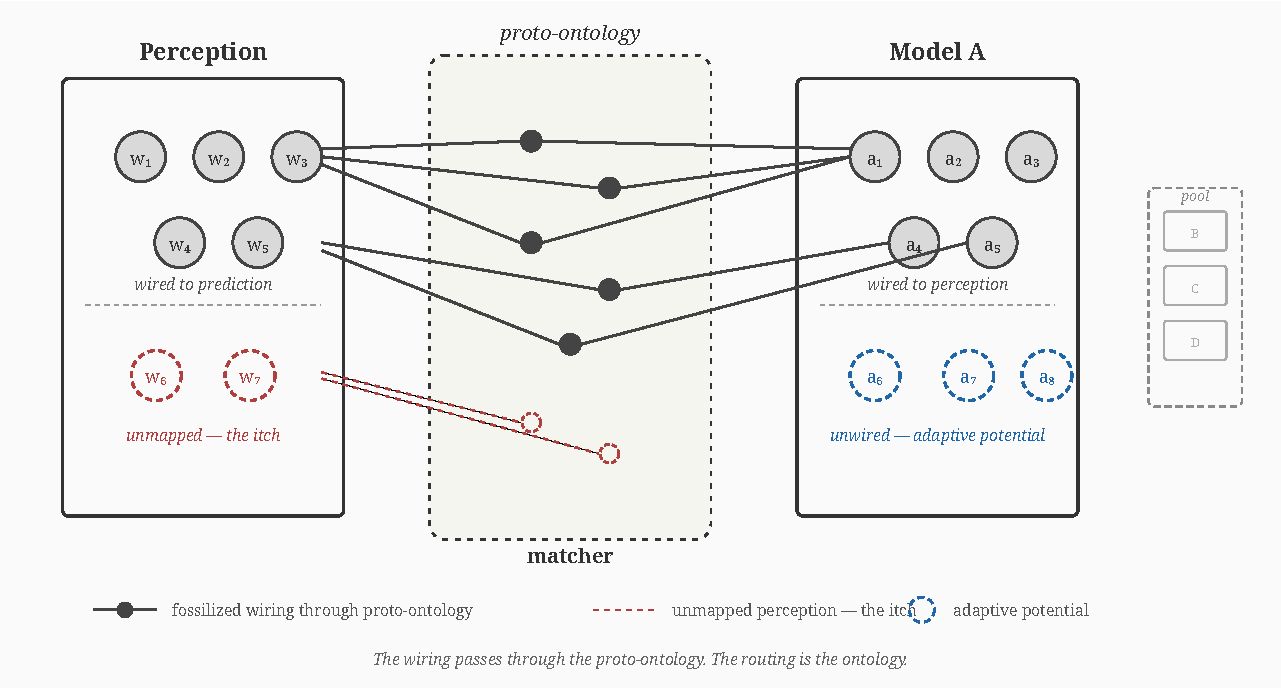
\includegraphics[width=0.7\textwidth]{architecture_diagram_v2}
  \caption{The three guiding signals in one frame: fossilized wiring
  (predictive error flows here), unmapped perception tokens (the itch),
  and unwired model capacity (adaptive potential).}
  \label{fig:architecture}
\end{figure}

In the course of experiments with implementing this architecture we
found it necessary to clearly articulate the three signals which drive
the system. The predictive error is the obvious one. But it turns out
to be insufficient on its own. When new token types begin to show up in
the perception stream, it may well be that the system can keep the
predictive error low by quietly ignoring them. The presence of unwired
perceptions needs to be a signal in itself. We call it the ``cognitive
itch,'' and the low reactivity to the itch is a sort of blindness.
Sudden occurrence of predictive error calls for a different reaction,
depending on the presence or absence of unwired perception tokens.
Coincidence of predictive error and new perceptions calls for extending
the current wirings, seeking to incorporate the new signals from the
world. Rise of the predictive error in absence of new perceptions calls
for radical rewiring and, concurrently, should trigger an active search
for any new perception tokens --- a frontier we have deferred in
Section~3. Likewise, the ``adaptive potential'' of the unwired pads of
a model does not affect the predictive error. But a wiring to a model
with some adaptive potential inherits this potential, which makes this
wiring valuable for reasons that are different from its current
predictive precision. Any wirings portfolio management strategy that
wants to account for adaptability needs to be aware of the adaptive
potential on top of the current predictive performance.

The origin and pre-selection of the predictive models portfolio, the
bootstrap under weak initial correlations, and the evolution of models
through fine-tuning once wired, are important practical concerns that
do not affect the architectural principles. We touch upon these issues
in Section~8.

\section{Computational Landscape}

\textbf{Helmholtz machine.} The Helmholtz machine \cite{dayan1995} calls
for two complementary but separate regimes of operation: a recognition
model and a generative model. It is clear that a full cognitive
architecture must cover both inference and exploitation. In this paper
we are focused on fleshing out some details of a possible inference
process. The fossilization does provide a point of support for a
potential switch between the operational modes.

\textbf{Bayesian program learning.} Lake, Salakhutdinov, and Tenenbaum
\cite{lake2015} learn compositional generative programs from few
examples. BPL shares our emphasis on structured representations and
sparse-data learning. Our program is more ambitious in the sense that
the hypothesis space is not directly prescribed, but is much more modest
in the sense that at this point we are concerned with signal routing
rather than signal formatting. We feel that many detailed aspects of
the architecture will benefit from probabilistic treatment once the
foundations are stable.

\textbf{Predictive processing.} The free energy framework
\cite{friston2010} and the broader predictive processing program
\cite{clark2013} share the principle that prediction error is the
fundamental cognitive signal. These architectures are rich, hierarchical,
and inspiring. Their focus is on the exploitation. Our architecture is
focused on inference. Prediction error evaluates candidate wirings
between systems rather than refining signal processing. Our program
seems complementary. We are deferring the frontier of how top-down
modulation fits into the architecture.

\textbf{Global Workspace Theory.} Baars \cite{baars1988} and its
computational extensions \cite{dehaene2011} propose a shared workspace
through which specialized processors broadcast information. Our
perception stream bears a surface resemblance to this workspace. The
difference: in GWT, the workspace is a communication channel from which
processors deposit and retrieve information. In our architecture, the
perception stream carries no meaning until the matching process gives
it one. It is raw material, not a message board.

\section{Theoretical Positioning}

Several behaviors of the architecture correspond tightly with established
ideas in cognitive science. These correspondences are double-edged: they
demonstrate possible mechanistic realizations, but at the same time
bring to light their mechanical constraints.

\textbf{Millikan.} As already stated in Section~4, the
ontology-as-wiring resulting from an interactive process is the
architecture's version of Millikan's teleosemantics \cite{millikan1984}.
The wiring process is constructive, offering some insight into how
teleosemantic relations can actually arise. Conversely, Millikan's
theory tells us how to think about the wirings, embedding the
architecture into the body of core cognitive science.

\textbf{Gopnik / Carey.} Looked at through the lens of Gopnik and
Carey's theory-theory \cite{gopnik1997, carey2009}, a specific wiring
between a specific model and the perception becomes ``a theory about the
world.'' The succession becomes the theory change. The ``hypothesis
testing'' is realized by an explicit, mechanistic process. The
conceptual repertoire, coming from available models and possible wirings,
is still pre-determined, but indirectly. And the architecture offers an
interesting staging to the repertoire extensions: learn new models, find
new applications. The succession dynamics described in Section~5 provide
a concrete mechanism for what Gopnik and Carey describe as theory change.

\textbf{Fodor.} A wired model, an established theory of the world,
generating predictions by driving an automaton --- this is as close to
Fodor's vision \cite{fodor2004} as a simple architecture can get. But
the wirings are not externally provided, and finding them makes
``concepts'' operational, not static symbols.

\section{Open Problems}

\textbf{From framework to theory.} The architecture, as implemented in
a minimalistic setup described in the companion paper, has generated
results that surprised its author. Whether it can do the same for an
independent reader is the threshold between framework and theory. This
paper is an invitation to test that.

\noindent\textbf{Conditions for failure.} It is possible, and actually probable,
that neither the matching process, nor the bootstrap process, are
successful. There could be worlds to which the simplistic mind of the
architecture cannot meaningfully relate, given a specific initial model
portfolio. We can only say that the overarching goal of the architecture
is not to eliminate the need for the innate, but to search for ways to
minimize it, to find a lower bound for what is known a priori which
still allows for a successful bootstrap.

\noindent\textbf{Perception granularity.} The architecture as presented assumes
unsupervised perception produces categories at the right granularity for
available models. This assumption is not categorical, it is tactical and
allows the presentation to be tractable. Sitting at the crossroads of
prediction and perception, cognition can and should be detecting and
signalling the success or the lack of it both up and down. We hope to
follow this trajectory, but only after consolidating the current scope.

\noindent\textbf{Inter-model consistency and complementarity.} We have only
hinted at inter-model consistency checks and their possible role in
mitigating the risks of model succession, and we have not discussed
complementary wirings at all. We consider these to be the scope of
future work, where actual modelling can give enough substance for the
proper treatment.

\noindent\textbf{Commitment under partial information.} A wiring that predicts
well locally may not generalize. The architecture's response to
incorrect fossilization is not prevention but correction --- succession
provides the mechanism for displacing an incumbent wiring when its
predictive power degrades. The quality of the correction depends on the
contender pool and the signal structure. In fact, the available
perception stream is always finite, and the prediction almost certainly
is never perfect. So a valid question is: under what criteria is the
matching process actually resolved? This is the finite-horizon decision
problem at the heart of real-time operation. It is our view that,
because such criteria are pragmatic in nature, it would be perilous to
tackle this problem before studying some working simulations.

\noindent\textbf{Temporal alignment.} The current implementation assumes one-step
temporal alignment between prediction and perception. Relaxing this
assumption introduces a temporal search dimension that compounds the
matching. We note the problem and defer it.

\noindent\textbf{The bootstrap and model fine-tuning.} Another valid question is
the origin of the predictive machinery. We could avoid this question
altogether, but let us share our experimentation-driven conjecture: the
architecture does require a pool of pre-existing predictive models from
which candidates are pre-selected based on initial fit to the perception
stream. It is not guaranteed that a strongly correlating wiring can be
found with the initial model portfolio. But even in case of weak initial
correlations the best-performing models and wirings are selected, and
fine-tuned through a bootstrap period. If the bootstrap process is
successful, the system eventually achieves a degree of predictive
success even when no initial model fits immediately. It is not a
first-order architectural issue and is not worked out in detail. Actual
simulations are the proper way to work out correct operational details.

\section{Conclusion}

The architecture, as presented here, is a result of trying to implement
a high-level idea in actual code. At many points in the process we felt
our hand being forced. The independence constraint has forced a matching
problem. The matching problem has forced an intermediate substrate.
Successful matching has produced a problem of retaining its outcome ---
hence fossilization. This gives us a sense of confidence in the
architecture, but a specific one: what works, works, maybe at the price
of missing some broader perspective. The perspective may be narrowing,
but ontological shift becomes inspectable, which is a deal we take.

\section*{Final Notes}

``Fossilized wiring'' as a term openly borrows from Selinker's
``fossilized errors'' \cite{selinker1972}. However, we would like to
note that here ``fossilization'' acquires a positive spin, which it
deserves.

The architecture is verifiably productive in the sense that we know at
least one theatrical play, \textit{Dogg's Hamlet} by Tom Stoppard
\cite{stoppard1979}, that hinges on its very principles. Stoppard wrote
it in 1979, which is a notable foresight.

The architecture was developed in conversation with large language
models, which served as both thinking partners and experimental
substrates (as they were quick to realize).

We have not been able to escape the biological and anthropocentric
undertones. ``Minimizing the innate'' is, of course, self-reflective,
and it is the original fuel for our effort.

\begin{thebibliography}{99}

\bibitem{companion}
[Companion paper — link to be added upon publication.]

\bibitem{baars1988}
Baars, B.~J. (1988). \textit{A Cognitive Theory of Consciousness}.
Cambridge University Press.

\bibitem{carey2009}
Carey, S. (2009). \textit{The Origin of Concepts}. Oxford University
Press.

\bibitem{clark2013}
Clark, A. (2013). Whatever next? Predictive brains, situated agents,
and the future of cognitive science. \textit{Behavioral and Brain
Sciences}, 36(3), 181--204.

\bibitem{dayan1995}
Dayan, P., Hinton, G.~E., Neal, R.~M., \& Zemel, R.~S. (1995). The
Helmholtz machine. \textit{Neural Computation}, 7(5), 889--904.

\bibitem{dehaene2011}
Dehaene, S., \& Changeux, J.~P. (2011). Experimental and theoretical
approaches to conscious processing. \textit{Neuron}, 70(2), 200--227.

\bibitem{fodor2004}
Fodor, J.~A. (2004). \textit{Hume Variations}. Oxford University Press.

\bibitem{friston2010}
Friston, K. (2010). The free-energy principle: a unified brain theory?
\textit{Nature Reviews Neuroscience}, 11(2), 127--138.

\bibitem{gopnik1997}
Gopnik, A., \& Meltzoff, A.~N. (1997). \textit{Words, Thoughts, and
Theories}. MIT Press.

\bibitem{harnad1990}
Harnad, S. (1990). The symbol grounding problem. \textit{Physica D},
42(1--3), 335--346.

\bibitem{kuhn1962}
Kuhn, T.~S. (1962). \textit{The Structure of Scientific Revolutions}.
University of Chicago Press.

\bibitem{lake2015}
Lake, B.~M., Salakhutdinov, R., \& Tenenbaum, J.~B. (2015). Human-level
concept learning through probabilistic program induction.
\textit{Science}, 350(6266), 1332--1338.

\bibitem{marr1982}
Marr, D. (1982). \textit{Vision}. W.~H. Freeman.

\bibitem{millikan1984}
Millikan, R.~G. (1984). \textit{Language, Thought, and Other Biological
Categories}. MIT Press.

\bibitem{piaget1952}
Piaget, J. (1952). \textit{The Origins of Intelligence in Children}.
International Universities Press.

\bibitem{quine1951}
Quine, W.~V.~O. (1951). Two dogmas of empiricism. \textit{Philosophical
Review}, 60(1), 20--43.

\bibitem{selinker1972}
Selinker, L. (1972). Interlanguage. \textit{International Review of
Applied Linguistics}, 10(3), 209--231.

\bibitem{stoppard1979}
Stoppard, T. (1979). \textit{Dogg's Hamlet, Cahoot's Macbeth}. Samuel
French.


\end{thebibliography}

\end{document}
